%%%%%%%%%%%%%%%%%%%%%%%%%%%%%%%%%%%%%%%%%
% Wenneker Assignment
% LaTeX Template
% Version 2.0 (12/1/2019)
%
% This template originates from:
% http://www.LaTeXTemplates.com
%
% Authors:
% Vel (vel@LaTeXTemplates.com)
% Frits Wenneker
%
% License:
% CC BY-NC-SA 3.0 (http://creativecommons.org/licenses/by-nc-sa/3.0/)
% 
%%%%%%%%%%%%%%%%%%%%%%%%%%%%%%%%%%%%%%%%%

%----------------------------------------------------------------------------------------
%	PACKAGES AND OTHER DOCUMENT CONFIGURATIONS
%----------------------------------------------------------------------------------------

\documentclass[11pt]{scrartcl} % Font size

%%%%%%%%%%%%%%%%%%%%%%%%%%%%%%%%%%%%%%%%%
% Wenneker Assignment
% Structure Specification File
% Version 2.0 (12/1/2019)
%
% This template originates from:
% http://www.LaTeXTemplates.com
%
% Authors:
% Vel (vel@LaTeXTemplates.com)
% Frits Wenneker
%
% License:
% CC BY-NC-SA 3.0 (http://creativecommons.org/licenses/by-nc-sa/3.0/)
% 
%%%%%%%%%%%%%%%%%%%%%%%%%%%%%%%%%%%%%%%%%

%----------------------------------------------------------------------------------------
%	PACKAGES AND OTHER DOCUMENT CONFIGURATIONS
%----------------------------------------------------------------------------------------

\usepackage{amsmath, amsfonts, amsthm} % Math packages

\usepackage{listings} % Code listings, with syntax highlighting

\usepackage[english]{babel} % English language hyphenation

\usepackage{graphicx} % Required for inserting images
\usepackage{caption}
\graphicspath{{Figures/}{./}} % Specifies where to look for included images (trailing slash required)

\usepackage{booktabs} % Required for better horizontal rules in tables

\numberwithin{equation}{section} % Number equations within sections (i.e. 1.1, 1.2, 2.1, 2.2 instead of 1, 2, 3, 4)
\numberwithin{figure}{section} % Number figures within sections (i.e. 1.1, 1.2, 2.1, 2.2 instead of 1, 2, 3, 4)
\numberwithin{table}{section} % Number tables within sections (i.e. 1.1, 1.2, 2.1, 2.2 instead of 1, 2, 3, 4)

\setlength\parindent{0pt} % Removes all indentation from paragraphs

\usepackage{enumitem} % Required for list customisation
\setlist{noitemsep} % No spacing between list items

%----------------------------------------------------------------------------------------
%	DOCUMENT MARGINS
%----------------------------------------------------------------------------------------

\usepackage{geometry} % Required for adjusting page dimensions and margins

\geometry{
	paper=a4paper, % Paper size, change to letterpaper for US letter size
	top=2.5cm, % Top margin
	bottom=3cm, % Bottom margin
	left=3cm, % Left margin
	right=3cm, % Right margin
	headheight=0.75cm, % Header height
	footskip=1.5cm, % Space from the bottom margin to the baseline of the footer
	headsep=0.75cm, % Space from the top margin to the baseline of the header
	%showframe, % Uncomment to show how the type block is set on the page
}

%----------------------------------------------------------------------------------------
%	FONTS
%----------------------------------------------------------------------------------------

\usepackage[utf8]{inputenc} % Required for inputting international characters
\usepackage[T1]{fontenc} % Use 8-bit encoding

\usepackage{fourier} % Use the Adobe Utopia font for the document

%\usepackage[framed,numbered,autolinebreaks,useliterate]{mcode}

%----------------------------------------------------------------------------------------
%	SECTION TITLES
%----------------------------------------------------------------------------------------

\usepackage{sectsty} % Allows customising section commands

\sectionfont{\normalfont\bfseries} % \section{} styling
\subsectionfont{\normalfont\bfseries} % \subsection{} styling
\subsubsectionfont{\normalfont\itshape} % \subsubsection{} styling
\paragraphfont{\normalfont\scshape} % \paragraph{} styling

%----------------------------------------------------------------------------------------
%	HEADERS AND FOOTERS
%----------------------------------------------------------------------------------------

\usepackage{scrlayer-scrpage} % Required for customising headers and footers

\ohead*{} % Right header
\ihead*{} % Left header
\chead*{} % Centre header

\ofoot*{} % Right footer
\ifoot*{} % Left footer
\cfoot*{\pagemark} % Centre footer

% MY PACKAGES
%\usepackage[framed,numbered,autolinebreaks,useliterate]{mcode}
\usepackage{listings}
\usepackage{float}
\usepackage{amsmath}
\usepackage{tikz}
\usetikzlibrary{shapes,arrows,positioning}
\usepackage{hyperref} % Include the file specifying the document structure and custom commands

%----------------------------------------------------------------------------------------
%	TITLE SECTION
%----------------------------------------------------------------------------------------

\title{	
	\normalfont\normalsize
	\textsc{Universität Würzburg}\\ % Your university, school and/or department name(s)
	\vspace{25pt} % Whitespace
	\rule{\linewidth}{0.5pt}\\ % Thin top horizontal rule
	\vspace{20pt} % Whitespace
	{\huge Übung 6}\\ % The assignment title
	{\Large Vorfilter, Regelabweichung und Ausgangsrückführung}\\
	\vspace{12pt} % Whitespace
	\rule{\linewidth}{2pt}\\ % Thick bottom horizontal rule
	\vspace{12pt} % Whitespace
}

\author{\LARGE Alexander Björk, Janis Kaltenthaler} % Your name

\date{\normalsize\today} % Today's date (\today) or a custom date

\begin{document}

\maketitle % Print the title

\tikzstyle{block} = [draw, fill=blue!20, rectangle, 
    minimum height=3em, minimum width=6em]
\tikzstyle{sum} = [draw, fill=blue!20, circle, node distance=1cm]
\tikzstyle{input} = [coordinate]
\tikzstyle{output} = [coordinate]
\tikzstyle{pinstyle} = [pin edge={to-,thin,black}]
\newcommand{\inte}{$\displaystyle \int$}

\section*{Aufgabe 6-1. Zustandsrückführung und Vorfilter (7 Punkte)}
\subsection*{a)}
Die bleibende Regelabweichung $e(\infty)$ für eine sprungförmige Führungsgröße $w(\infty)=1$ berechnet sich wie folgt:
\begin{align*}
	e(\infty)&=w(\infty)-y(\infty)=w(\infty)+C(A-BK)^{-1}Bw(\infty)\\
	e(\infty)&=(I+C(A-BK)^{-1}B)w(\infty)\\
	e(\infty)&=\Biggl(1+\begin{bmatrix}1&0\end{bmatrix}\begin{bmatrix}0&1\\-5&-2\end{bmatrix}^{-1}\begin{bmatrix}0\\0.5\end{bmatrix}\Biggr)\cdot 1=0.9
\end{align*}
\subsection*{b)}
Der Vorfilter $V$ berechnet sich nun wie folgt:
\begin{align*}
	V&=-(C(A-BK)^{-1}B)^{-1}=-\Biggl(\begin{bmatrix}1&0\end{bmatrix}\begin{bmatrix}0&1\\-5&-2\end{bmatrix}^{-1}\begin{bmatrix}0\\0.5\end{bmatrix}\Biggr)^{-1}\\
	V&=10
\end{align*}
Durch den Vorfilter ändert sich das Zustandsraummodell zu:
\begin{align*}
	\dot{x}(t)&=\begin{bmatrix}0&1\\-5&-2\end{bmatrix}x(t)+\begin{bmatrix}0\\5\end{bmatrix}w(t)+\begin{bmatrix}0\\0.25\end{bmatrix}d(t)\hspace{20pt} x(0)=x_0\\
	y(t)&=\begin{bmatrix}1&0\end{bmatrix}x(t)
\end{align*}
\subsection*{c)}
Die Berechnung der bleibenden Regelabweichung ohne Störgröße folgt dem selben Prinzip wie in Teilaufgabe \textbf{a)}:
\begin{align*}
	e(\infty)&=w(\infty)-y(\infty)=w(\infty)+C(A-BK)^{-1}Bw(\infty)\\
	e(\infty)&=(I+C(A-BK)^{-1}B)w(\infty)\\
	e(\infty)&=\Biggl(1+\begin{bmatrix}1&0\end{bmatrix}\begin{bmatrix}0&1\\-5&-2\end{bmatrix}^{-1}\begin{bmatrix}0\\5\end{bmatrix}\Biggr)\cdot 1=0
\end{align*}
Druch den Vorfilter konnte die bleibende Regelabweichung eliminiert werden. Wirkt nun jedoch zusätzlich eine sprungförmige Störgröße $d(\infty)=1$, ändert sich die Berechnungsvorschrift für die bleibende Regelabweichung wie folgt:
\begin{align*}
	e(\infty)&=w(\infty)-y(\infty)=w(\infty)+C(A-BK)^{-1}Bw(\infty)+C(A-BK)^{-1}Ed(\infty)\\
	e(\infty)&=1+\begin{bmatrix}1&0\end{bmatrix}\begin{bmatrix}0&1\\-5&-2\end{bmatrix}^{-1}\begin{bmatrix}0\\5\end{bmatrix}\cdot 1+\begin{bmatrix}1&0\end{bmatrix}\begin{bmatrix}0&1\\-5&-2\end{bmatrix}^{-1}\begin{bmatrix}0\\0.25\end{bmatrix}\cdot 1\\
	e(\infty)&=-0.05
\end{align*}
Für eine Störung $d(t)\neq 0$ ergibt sich stets eine bleibende Regelabweichung, d.h. $e(\infty)\neq 0$.

\subsection*{d)}
\begin{figure}[H]
\centering
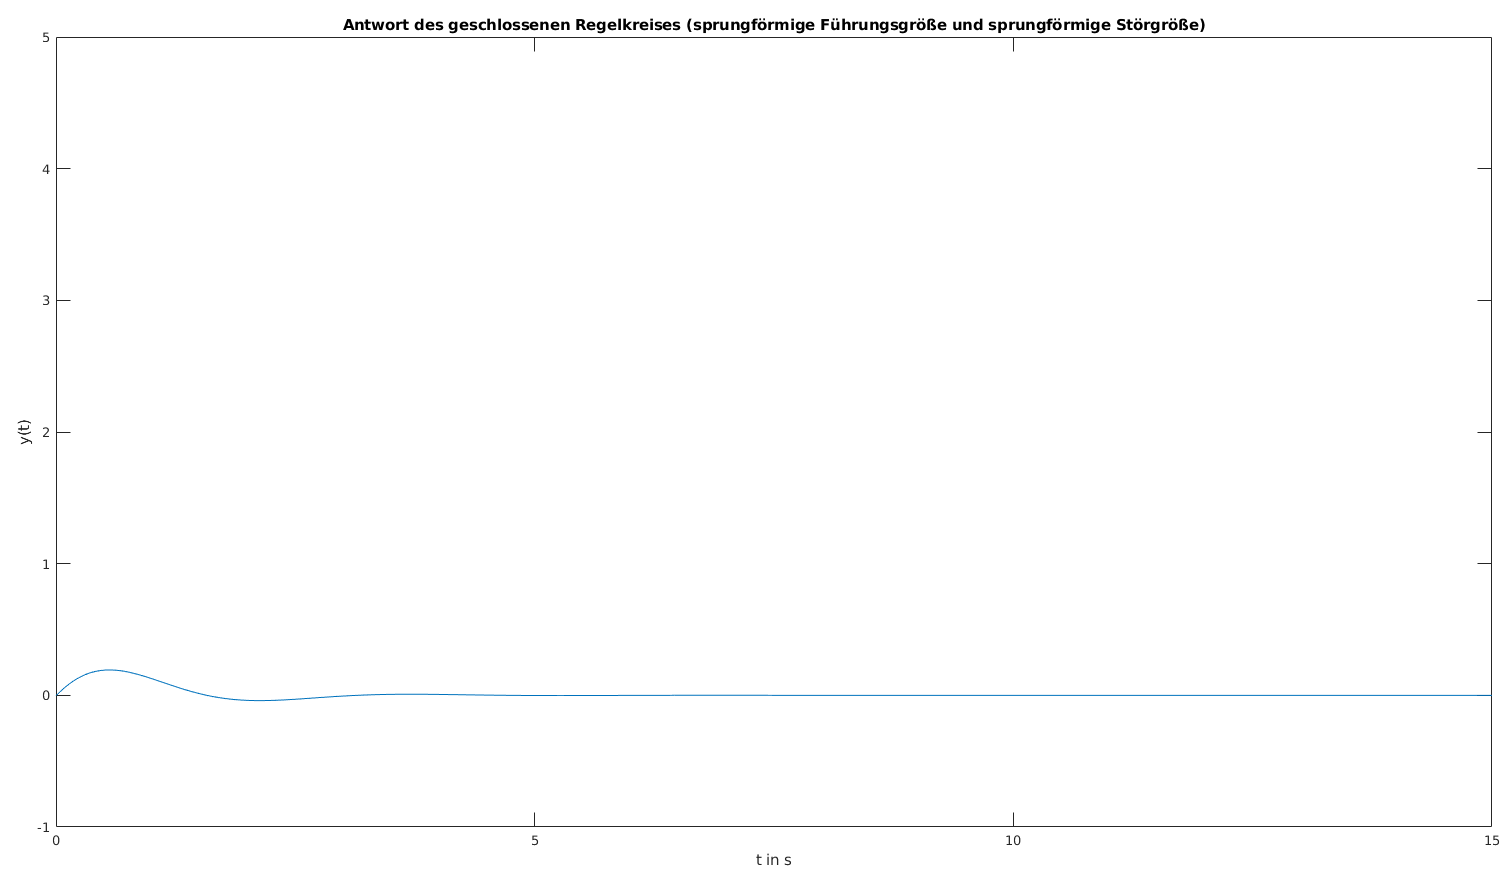
\includegraphics[width=\textwidth]{sprung_sprung.png}
\captionsetup{labelformat=empty}
\caption{Abb. 6-1.1: Antwort des geschlossenen Regelkreises für den Fall einer sprungförmigen Führungsgröße $w$ und einer sprungförmigen Störgröße $d$.}
\end{figure}

\begin{figure}[H]
\centering
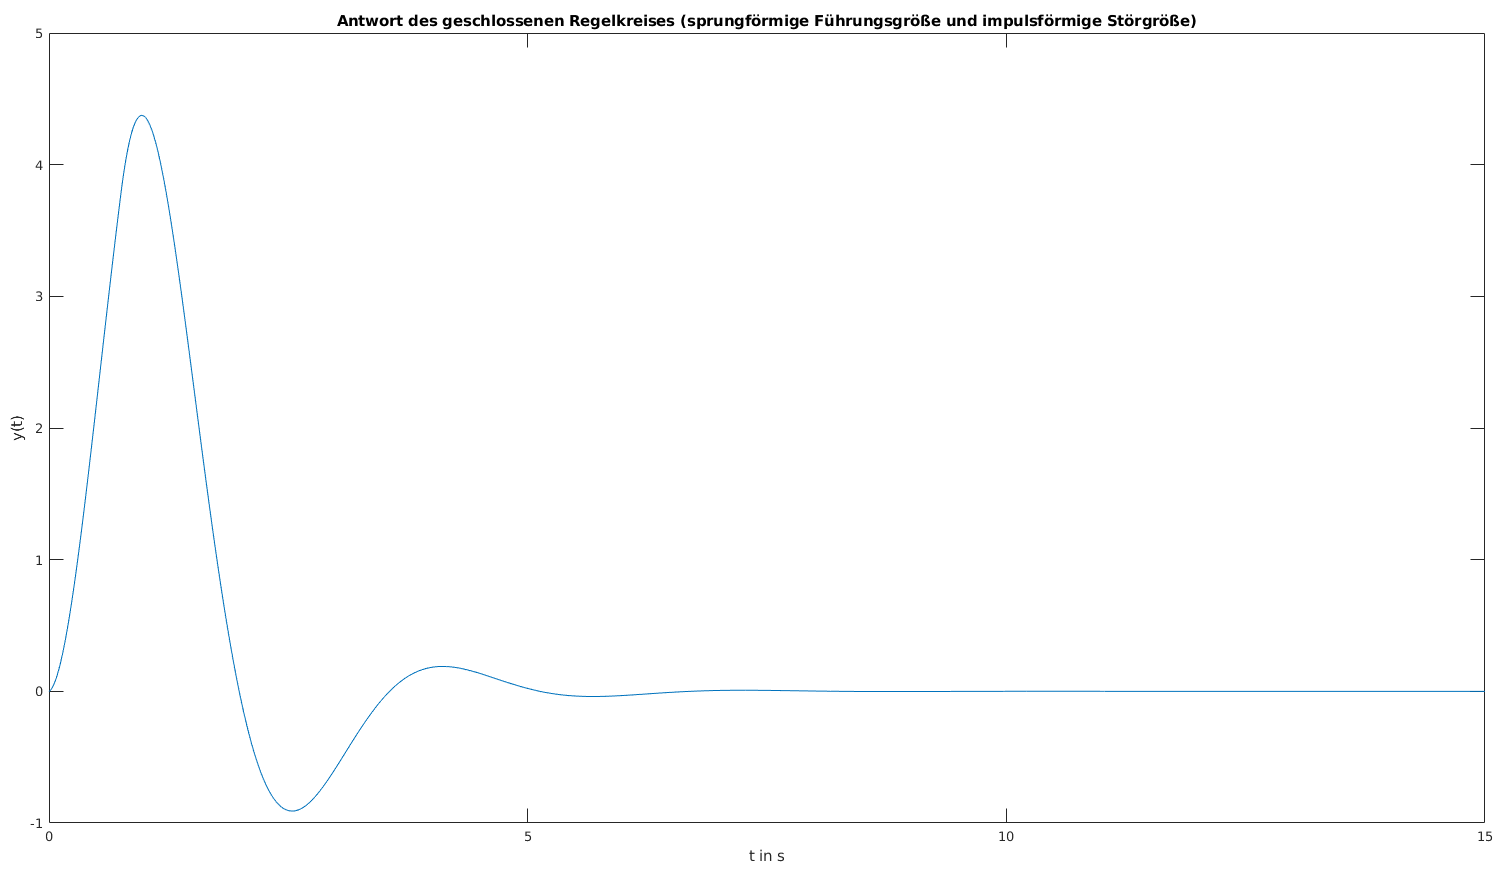
\includegraphics[width=\textwidth]{sprung_impuls.png}
\captionsetup{labelformat=empty}
\caption{Abb. 6-1.2: Antwort des geschlossenen Regelkreises für den Fall einer sprungförmigen Führungsgröße $w$ und einer impulsförmigen Störgröße $d$.}
\end{figure}

\section*{6-2: Ackermann-Formel (3 Punkte)}
Die Ackerman-Formel ergibt sich zuallererst aus der Umstellung zu
\begin{align*}
k^T &= k_R^TT_R^{-1} = \left( \begin{pmatrix}
\bar{a}_0 & \bar{a}_1 & \hdots & \bar{a}_{n-1}
\end{pmatrix} - \begin{pmatrix}
a_0 & a_1 & \hdots & a_{n-1}
\end{pmatrix} 
\right) T_R^{-1}.
\end{align*}
Anschließend wird die Transformationsmatrix
\begin{align*}
T_R^{-1} &= \begin{pmatrix}
s_R^T \\
s_R^TA \\
\vdots \\
s_R^TA^{n-1}
\end{pmatrix}
\end{align*}
direkt eingesetzt, um eine extra Berechnung zu vermeiden:
\begin{align*}
k^T=\begin{pmatrix}
\bar{a}_0 & \bar{a}_1 & \hdots & \bar{a}_{n-1}
\end{pmatrix} \begin{pmatrix}
s_R^T \\
s_R^TA \\
\vdots \\
s_R^TA^{n-1}
\end{pmatrix} - \underbrace{\begin{pmatrix}
a_0 & a_1 & \hdots & a_{n-1}
\end{pmatrix} \begin{pmatrix}
s_R^T \\
s_R^TA \\
\vdots \\
s_R^TA^{n-1}
\end{pmatrix}}_{=-s_R^TA^n}
\end{align*}
Ausgeschrieben ergibt dies die Ackermann-Formel.
\begin{align*}
k^T &= \begin{pmatrix}
\bar{a}_0 & \bar{a}_1 & \bar{a}_2 & \hdots & \bar{a}_{n-1} & 1
\end{pmatrix} \begin{pmatrix}
s_R^T \\
s_R^TA \\
\vdots \\
s_R^TA^{n-1} \\
s_r^TA^n
\end{pmatrix} \\
k^T &= s_R^T \left( \bar{a}_0\textit{\textbf{I}} + \bar{a}_1\textit{\textbf{A}} + \bar{a}_2\textit{\textbf{A}}^2 +  \hdots + \bar{a}_{n-1}\textit{\textbf{A}}^{n-1} + \textbf{\textit{A}}^n \right)
\end{align*}

\section*{6-3: Ausgangsrückführung (3 Punkte)}
\subsection*{a)}
Das resultierende ZMR ist
\begin{align*}
\dot{x}(t) &= \begin{bmatrix}
-26 &  20 \\
-30 &  23
\end{bmatrix} x(t) + \begin{bmatrix}
1 \\ 1
\end{bmatrix} u(t) \\
y(t) &= \begin{bmatrix}
-9 & 7
\end{bmatrix} x(t)
\end{align*}
mit
\begin{align*}
K = \begin{bmatrix}
27 & -21
\end{bmatrix}
\end{align*}

\subsection*{b)}
Das resultierende ZMR ist
\begin{align*}
\dot{x}(t) &= \begin{bmatrix}
-26 &  20 \\
-30 &  23
\end{bmatrix} x(t) + \begin{bmatrix}
1 \\ 1
\end{bmatrix} u(t) \\
y(t) &= \begin{bmatrix}
-9 & 7
\end{bmatrix} x(t)
\end{align*}
mit
\begin{align*}
K_y = -3
\end{align*}

\end{document}
